\documentclass[aspectratio=169,10pt]{beamer}
% =====================================================================
%  Le Collé — thème de présentation (même palette et mêmes notations que la fiche)
% =====================================================================
\usepackage[utf8]{inputenc}
\usepackage[T1]{fontenc}
\usepackage[sc]{mathpazo}
\usepackage[scaled=0.92]{helvet}
\usefonttheme{professionalfonts}
\usepackage{amsmath,amssymb,mathrsfs,stmaryrd}
\usepackage{microtype}
\usepackage{booktabs,array,multicol}
\usepackage[most]{tcolorbox}
\usepackage{tikz,pgfplots}
\usetikzlibrary{arrows.meta,calc,positioning,decorations.pathreplacing,shapes.misc}
\pgfplotsset{compat=1.17,trig format plots=rad}
\usepackage{tkz-tab}

% ---------- palette (identique à la fiche) ----------
\definecolor{Ink}{HTML}{1C2533}\definecolor{Bleu}{HTML}{1F3A5F}\definecolor{BleuMoyen}{HTML}{4A6A8F}
\definecolor{BleuClair}{HTML}{9DB2C9}\definecolor{Fond}{HTML}{F2F4F7}\definecolor{Ocre}{HTML}{B07A26}
\definecolor{Brique}{HTML}{A23B2A}\definecolor{Gris}{HTML}{5E6672}\definecolor{Filet}{HTML}{C5CCD6}
\definecolor{Vert}{HTML}{2E6B4F}

% ---------- notations (identiques à la fiche) ----------
\newcommand{\K}{\mathbb{K}}\newcommand{\R}{\mathbb{R}}\newcommand{\C}{\mathbb{C}}\newcommand{\Z}{\mathbb{Z}}
\newcommand{\Mn}[1]{\mathcal{M}_{n}(#1)}\newcommand{\rg}{\operatorname{rg}}\newcommand{\vect}{\operatorname{Vect}}
\newcommand{\Mat}{\operatorname{Mat}}\newcommand{\Id}{\operatorname{Id}}\newcommand{\com}{\operatorname{com}}
\newcommand{\vv}[1]{\overrightarrow{#1}}\newcommand{\ve}[1]{\vec{#1}}
\newcommand{\dt}[1]{\left|\begin{matrix}#1\end{matrix}\right|}
\DeclareRobustCommand{\HP}{{\sffamily\bfseries\scriptsize\textcolor{Brique}{[HP]}}}

% ---------- réglages beamer ----------
\setbeamertemplate{navigation symbols}{}
\setbeamersize{text margin left=0.85cm,text margin right=0.85cm}
\setbeamercolor{normal text}{fg=Ink,bg=white}
\setbeamercolor{structure}{fg=Bleu}
\setbeamercolor{alerted text}{fg=Brique}
\setbeamerfont{alerted text}{series=\bfseries}
\setbeamertemplate{itemize item}{\raisebox{0.15em}{\textcolor{Ocre}{\rule{0.38em}{0.38em}}}}
\setbeamertemplate{itemize subitem}{\textcolor{BleuMoyen}{\scriptsize\textbullet}}
\setbeamertemplate{enumerate item}{\textcolor{Bleu}{\sffamily\bfseries\insertenumlabel.}}
\setlength{\leftmargini}{1.2em}
\setbeamertemplate{blocks}[default]

% numéro de la partie courante, rappelé dans le titre et le pied de page (renvoi à la fiche)
\def\fichesec{}\def\chapnom{}
\newcommand{\chapitre}[1]{\def\chapnom{#1}}

\setbeamertemplate{frametitle}{%
  \vskip0.28cm
  \ifx\fichesec\empty\else
    \tikz[baseline=(b.base)]\node[fill=Ocre,text=white,font=\sffamily\bfseries\scriptsize,inner sep=2.5pt,rounded corners=1pt](b){\fichesec};\hspace{0.45em}%
  \fi
  {\color{Bleu}\sffamily\bfseries\Large\insertframetitle}\par
  \vskip0.06cm{\color{Filet}\rule{\linewidth}{0.5pt}}\vskip-0.2cm}

\setbeamertemplate{footline}{%
  \hbox to\paperwidth{%
    \hspace*{0.85cm}{\scriptsize\sffamily\color{Gris}Le Collé\ \ \textcolor{Filet}{|}\ \ \chapnom}\hfill
    {\scriptsize\sffamily\color{Gris}\ifx\fichesec\empty\else fiche \textbf{\color{Ocre}§\fichesec}\quad\fi\insertframenumber}\hspace*{0.85cm}}%
  \vskip0.18cm
  \hbox{\begin{tikzpicture}
    \fill[Fond] (0,0) rectangle (\paperwidth,2.2pt);
    \pgfmathsetmacro\prog{min(\insertframenumber/max(\inserttotalframenumber,1),1)}
    \fill[Ocre] (0,0) rectangle ({\prog*\paperwidth},2.2pt);
  \end{tikzpicture}}}

% ---------- encadrés : même code couleur que la fiche ----------
\tcbset{sb/.style={enhanced,arc=1pt,boxrule=0pt,left=6pt,right=6pt,top=3pt,bottom=3pt,before skip=0.14cm,after skip=0.14cm,
  fontupper=\normalsize\raggedright}}
\newcommand{\etiq}[2]{{\sffamily\bfseries\scriptsize\color{#1}\MakeUppercase{#2}}\par\vspace{2pt}}
\newtcolorbox{DEF}[1][Définition]{sb,colback=white,borderline west={2pt}{0pt}{Bleu},before upper={\etiq{Bleu}{#1}}}
\newtcolorbox{PROP}[1][Propriété]{sb,colback=Fond,borderline west={3pt}{0pt}{Bleu},before upper={\etiq{Bleu}{#1}}}
\newtcolorbox{FORM}[1][Formule]{sb,colback=white,colframe=BleuMoyen,boxrule=0.6pt,before upper={\etiq{BleuMoyen}{#1}}}
\newtcolorbox{METH}[1]{sb,colback=white,borderline north={1pt}{0pt}{Bleu},borderline south={1pt}{0pt}{Bleu},
  before upper={{\sffamily\bfseries\scriptsize\colorbox{Bleu}{\color{white}MÉTHODE}\ \color{Bleu}#1}\par\vspace{3pt}}}
\newtcolorbox{PIEGE}[1][Piège]{sb,colback=Brique!6,borderline west={2pt}{0pt}{Brique},before upper={\etiq{Brique}{#1}}}
\newtcolorbox{ASTU}[1][Astuce]{sb,colback=Ocre!8,borderline west={2pt}{0pt}{Ocre},before upper={\etiq{Ocre}{#1}}}
\newtcolorbox{HPBOX}{sb,colback=white,borderline west={2pt}{0pt}{Brique},before upper={\etiq{Brique}{Hors programme}}}
\newtcolorbox{ATOI}[1][À toi]{sb,colback=Vert!6,borderline west={2pt}{0pt}{Vert},before upper={\etiq{Vert}{#1}}}
\newtcolorbox{RETENIR}{sb,colback=Bleu!5,colframe=Bleu,boxrule=0.8pt,left=8pt,
  before upper={\etiq{Bleu}{À retenir}}}
\newtcolorbox{EX}[1][Exemple]{sb,colback=white,colframe=Filet,boxrule=0.5pt,before upper={\etiq{Gris}{#1}}}

% complément pédagogique absent du livre : étiquette pointillée
\DeclareRobustCommand{\ajout}{\tikz[baseline=(a.base)]\node[draw=Gris,dashed,text=Gris,font=\sffamily\scriptsize,inner sep=2pt,rounded corners=1pt](a){complément hors livre};}
\DeclareRobustCommand{\livre}[1]{{\sffamily\scriptsize\color{Gris}[livre #1]}}
\newcommand{\rep}[1]{\textcolor{Vert}{#1}}% réponse attendue de l'élève

% ---------- styles de figures (identiques au livre) ----------
\pgfplotsset{courbe/.style={axis lines=middle,axis equal image,
  axis line style={Gris,-{Stealth[length=4pt]}},
  xlabel={$x$},ylabel={$y$},ticklabel style={font=\scriptsize\sffamily,color=Gris},
  every axis x label/.style={at={(ticklabel* cs:1)},anchor=west,font=\small},
  every axis y label/.style={at={(ticklabel* cs:1)},anchor=south,font=\small},
  samples=200,smooth}}
\pgfplotsset{mini/.style={axis lines=middle,axis line style={Filet},xtick=\empty,ytick=\empty,width=3.9cm,height=3.9cm,
  xmin=-1.15,xmax=1.15,ymin=-1.15,ymax=1.15,title style={font=\footnotesize\sffamily,yshift=-0.1cm},samples=100}}
\tikzset{arcetude/.style={Bleu,line width=1.25pt},
         reste/.style={BleuClair,line width=1pt},
         tgte/.style={Ocre,line width=1pt},
         asy/.style={Gris,dashed,line width=0.7pt},
         pt/.style={circle,fill=Ink,inner sep=1.3pt},
         >={Stealth[length=5pt]}}

% ---------- diapositives de partie ----------
% \partie{num}{titre}{question guide}{liste des parties du chapitre via \rm}
\newcommand{\rmitem}[2]{\def\tmp{#1}%
  \ifx\tmp\fichesec{\color{Bleu}\bfseries #1\quad #2}\else{\color{Gris!70}#1\quad #2}\fi\par\vspace{2pt}}
\newcommand{\partie}[4]{%
  \def\fichesec{#1}\section{#2}%
  \begin{frame}[plain]
  \begin{tikzpicture}[remember picture,overlay]
    \fill[Bleu] (current page.north west) rectangle ([xshift=6.3cm]current page.south west);
    \node[anchor=north west,text=white,font=\sffamily\bfseries\fontsize{40}{40}\selectfont] at ([xshift=0.8cm,yshift=-1.2cm]current page.north west) {#1};
    \node[anchor=north west,text width=4.8cm,align=left,text=white,font=\sffamily\bfseries\Large] at ([xshift=0.8cm,yshift=-2.9cm]current page.north west) {\hyphenpenalty=10000\exhyphenpenalty=10000 #2\par};
    \node[anchor=south west,text width=4.8cm,text=white!75!Bleu,font=\sffamily\scriptsize] at ([xshift=0.8cm,yshift=0.6cm]current page.south west) {\chapnom\\fiche \textbf{§#1}};
  \end{tikzpicture}
  \hspace*{5.5cm}\begin{minipage}{8.4cm}
  {\sffamily\scriptsize\color{Ocre}\bfseries LA QUESTION}\par\vspace{2pt}
  {\large #3}\par\vspace{0.7cm}
  {\sffamily\scriptsize\color{Gris}\bfseries DANS CE CHAPITRE}\par\vspace{4pt}
  {\sffamily\small #4}
  \end{minipage}
  \end{frame}}



% ---------- exercices en séance : énoncé sur une diapositive, correction sur la suivante ----------
\newcommand{\badgeexo}[1]{\tikz[baseline=(e.base)]\node[fill=Vert,text=white,font=\sffamily\bfseries\scriptsize,inner sep=2.5pt,rounded corners=1pt](e){EXERCICE #1};\hspace{0.4em}}
\newcommand{\badgecor}[1]{\tikz[baseline=(e.base)]\node[draw=Vert,line width=0.8pt,text=Vert,font=\sffamily\bfseries\scriptsize,inner sep=2.2pt,rounded corners=1pt](e){CORRECTION #1};\hspace{0.4em}}
\newtcolorbox{ENONCE}[1][]{sb,colback=Vert!6,borderline west={3pt}{0pt}{Vert},left=9pt,top=5pt,bottom=5pt,
  before upper={{\sffamily\bfseries\scriptsize\color{Vert}À TOI\ifx\relax#1\relax\else\ \ ·\ \ \MakeUppercase{#1}\fi}\par\vspace{4pt}}}
\newtcolorbox{INDICE}{sb,colback=white,colframe=Vert!60,boxrule=0.5pt,borderline={0.5pt}{0pt}{Vert!60,dashed},
  before upper={\etiq{Vert}{Indice (si besoin)}}}
\newtcolorbox{RAIS}[1][Le raisonnement]{sb,colback=Vert!5,borderline west={2pt}{0pt}{Vert},before upper={\etiq{Vert}{#1}}}
\newtcolorbox{OUTIL}{sb,colback=Fond,borderline west={2pt}{0pt}{Bleu},before upper={\etiq{Bleu}{Propriété ou méthode utilisée}}}
\newcommand{\etape}[1]{{\sffamily\bfseries\footnotesize\color{Vert}#1}\ }
\newcommand{\objectif}[1]{\par\vspace{2pt}{\footnotesize\sffamily\color{Gris}Objectif : #1}}
\newcommand{\sh}{\operatorname{sh}}\newcommand{\ch}{\operatorname{ch}}
\title{Le Collé --- Équations différentielles}

\begin{document}

% ---------------------------------------------------------------- titre
\begin{frame}[plain]
\begin{tikzpicture}[remember picture,overlay]
  \fill[Bleu] (current page.north west) rectangle (current page.south east);
  \node[anchor=north west,text=white!70!Bleu,font=\sffamily\scriptsize] at ([xshift=1cm,yshift=-1.2cm]current page.north west)
    {LE COLLÉ\ \ ·\ \ MATHÉMATIQUES PT\ \ ·\ \ CHAPITRE 4\ \ ·\ \ SUPPORT DE SÉANCE};
  \node[anchor=north west,text=white,font=\sffamily\bfseries\fontsize{26}{30}\selectfont,text width=13cm] at ([xshift=1cm,yshift=-2.1cm]current page.north west)
    {Équations différentielles\\ linéaires};
  \fill[Ocre] ([xshift=1cm,yshift=-4.6cm]current page.north west) rectangle ([xshift=4cm,yshift=-4.65cm]current page.north west);
  \node[anchor=north west,text=white!80!Bleu,font=\normalsize,text width=12.5cm] at ([xshift=1cm,yshift=-5cm]current page.north west)
    {Présentation pour expliquer, avec sept exercices à chercher en séance ;\\ le \textbf{livre} pour relire, la \textbf{fiche} pour réviser.
     Mêmes parties (§1.1 à §1.5), mêmes notations.};
\end{tikzpicture}
\end{frame}

% ---------------------------------------------------------------- mode d'emploi
\begin{frame}{Comment utiliser ce support}
\vspace{-0.15cm}
\begin{columns}[T]
\column{0.48\textwidth}
\begin{DEF}vocabulaire à connaître\end{DEF}\vspace{-9pt}
\begin{PROP}[Propriété / théorème]énoncé précis, avec ses hypothèses\end{PROP}\vspace{-9pt}
\begin{METH}{}démarche à suivre, étape par étape\end{METH}\vspace{-9pt}
\begin{PIEGE}erreur classique à éviter\end{PIEGE}
\column{0.48\textwidth}
\begin{ENONCE}[durée indicative]exercice à chercher en séance : diapositive \textbf{seule}, la correction est sur la suivante\end{ENONCE}\vspace{-9pt}
\begin{RAIS}correction : d'abord le raisonnement, puis la méthode, puis les étapes\end{RAIS}\vspace{-9pt}
\begin{ASTU}technique qui fait gagner du temps\end{ASTU}\vspace{-9pt}
\begin{RETENIR}l'essentiel d'une partie\end{RETENIR}
\end{columns}
{\footnotesize Les badges \badgeexo{1} et \badgecor{1} repèrent les exercices et leurs corrections. Le numéro ocre
\tikz[baseline=(b.base)]\node[fill=Ocre,text=white,font=\sffamily\bfseries\scriptsize,inner sep=2pt](b){1.2}; renvoie à la partie de la fiche.}
\end{frame}

% ---------------------------------------------------------------- plan
\begin{frame}{Plan de la séance (2 h)}
\begin{columns}[T]
\column{0.55\textwidth}
\small
\renewcommand{\arraystretch}{1.35}
\begin{tabular}{@{}l l r@{}}
\textbf{\color{Bleu}1.1} & Structure, théorème de Cauchy & \color{Vert}Ex.~1\\
\textbf{\color{Bleu}1.2} & Premier ordre, recollement & \color{Vert}Ex.~2, 3\\
\textbf{\color{Bleu}1.3} & Second ordre, coefficients constants & \color{Vert}Ex.~4, 5\\
\textbf{\color{Bleu}1.4} & Second ordre, coefficients continus & \color{Vert}Ex.~6, 7\\
\textbf{\color{Bleu}1.5} & Quelle méthode ? Synthèse &
\end{tabular}
\column{0.4\textwidth}
\begin{ASTU}[Rythme suggéré]
\small 1.1--1.2 : 45 min\\ 1.3 : 35 min\\ 1.4--1.5 : 40 min\\[3pt]
Chaque exercice : 3 à 8 min de recherche, puis la correction.
\end{ASTU}
\end{columns}
\vspace{0.2cm}
{\small\color{Gris}Après la séance : relire le livre, apprendre la fiche, puis les \textbf{cinq problèmes}, puis le TD.}
\end{frame}

\chapitre{Chapitre 4 · Équations différentielles}
\newcommand{\rmI}{\rmitem{1.1}{Structure, théorème de Cauchy}\rmitem{1.2}{Premier ordre, recollement}\rmitem{1.3}{Second ordre, coefficients constants}
  \rmitem{1.4}{Second ordre, coefficients continus}\rmitem{1.5}{Quelle méthode ? Synthèse}}

\begin{frame}[plain]
\begin{tikzpicture}[remember picture,overlay]
  \fill[Bleu] (current page.north west) rectangle (current page.south east);
  \fill[Ocre] ([yshift=-4.2cm]current page.north west) rectangle ([yshift=-4.25cm,xshift=5cm]current page.north west);
  \node[anchor=north west,text=white!70!Bleu,font=\sffamily\small] at ([xshift=1cm,yshift=-1.6cm]current page.north west) {Chapitre 4};
  \node[anchor=north west,text=white,font=\sffamily\bfseries\fontsize{30}{32}\selectfont] at ([xshift=1cm,yshift=-2.3cm]current page.north west) {Équations différentielles};
  \node[anchor=north west,text width=12.5cm,text=white,font=\large] at ([xshift=1cm,yshift=-4.7cm]current page.north west)
    {Une solution particulière, plus toutes les solutions sans second membre.\\[2pt]
     \normalsize\color{white!75!Bleu} Pour une équation linéaire, l'ensemble des solutions est une droite ou un plan « déplacé ».
     Tout le chapitre consiste à trouver ce plan, puis un seul point.};
\end{tikzpicture}
\end{frame}

% =====================================================================
\partie{1.1}{Structure, théorème de Cauchy}{Pourquoi suffit-il de trouver deux solutions, et une seule solution particulière ?}{\rmI}

\begin{frame}{D'où viennent ces équations ?}
\begin{columns}[T]
\column{0.5\textwidth}
\textbf{Circuit RC} soumis à une tension $e(t)$ :
\[q'(t)+\frac1{RC}\,q(t)=\frac{e(t)}R.\]
\textbf{Oscillateur} (masse, ressort, frottement) :
\[x''(t)+2\lambda x'(t)+\omega^2x(t)=f(t).\]
\pause
\begin{itemize}
\item l'inconnue est une \alert{fonction} ;
\item elle et ses dérivées apparaissent \alert{au premier degré} : l'équation est \emph{linéaire} ;
\item le membre de droite (le « forçage ») est le \emph{second membre}.
\end{itemize}
\column{0.45\textwidth}
\centering
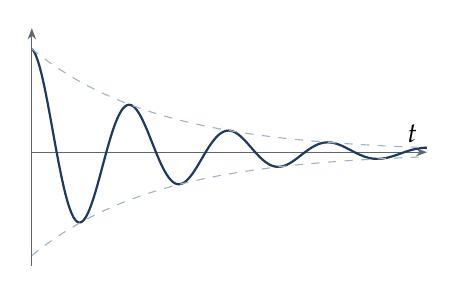
\begin{tikzpicture}
\begin{axis}[width=6.6cm,height=4.6cm,axis lines=middle,xmin=0,xmax=12.5,ymin=-1.1,ymax=1.2,xtick=\empty,ytick=\empty,
  axis line style={Gris,-{Stealth[length=4pt]}},samples=200,xlabel={$t$}]
\addplot[Bleu,thick,domain=0:12.5]{exp(-0.25*x)*cos(2*x)};
\addplot[BleuClair,dashed,domain=0:12.5]{exp(-0.25*x)};
\addplot[BleuClair,dashed,domain=0:12.5]{-exp(-0.25*x)};
\end{axis}
\end{tikzpicture}\\
{\footnotesize\color{Gris}oscillateur amorti, sans forçage}
\end{columns}
\end{frame}

\begin{frame}{Définition et forme normalisée}
\begin{DEF}
$I$ intervalle, $a,b,c$ \alert{continues} sur $I$ à valeurs dans $\K=\R$ ou $\C$.
\[(E)\quad y'+a(t)y=b(t)\qquad\text{ou}\qquad(E)\quad y''+a(t)y'+b(t)y=c(t).\]
Solution : fonction dérivable (deux fois dérivable) sur $I$ qui vérifie $(E)$ \emph{en tout point de $I$}.
$(H)$ : l'équation \emph{homogène} associée (second membre remplacé par $0$).
\end{DEF}
\pause
\begin{PIEGE}[Normaliser, sur un intervalle]
$\alpha(t)y''+\beta(t)y'+\gamma(t)y=\delta(t)$ : on divise par $\alpha(t)$ \alert{seulement sur un intervalle où $\alpha$ ne s'annule
pas}. Exemple : $ty'+y=\ln t$ se normalise sur $\R_+^*$ en $y'+\frac1ty=\frac{\ln t}t$. Les points où $\alpha$ s'annule : §1.2, recollement.
\end{PIEGE}
\end{frame}

\begin{frame}{La structure : un plan « déplacé »}
\begin{columns}[c]
\column{0.57\textwidth}
\begin{PROP}[Structure \livre{prop.~1.2}]
$L(y)=y''+a(t)y'+b(t)y$ est \emph{linéaire}.
\begin{enumerate}
\item $S_H=\mathrm{Ker}\,L$ est un espace vectoriel.
\item Superposition : $L(y_1)=c_1$, $L(y_2)=c_2\Rightarrow L(y_1+y_2)=c_1+c_2$.
\item Si $y_p$ est une solution de $(E)$ : \quad $S_E=y_p+S_H$.
\end{enumerate}
\end{PROP}
\pause
Preuve du 3 : $L(y)=c=L(y_p)\iff L(y-y_p)=0\iff y-y_p\in S_H$.
\column{0.4\textwidth}
\centering
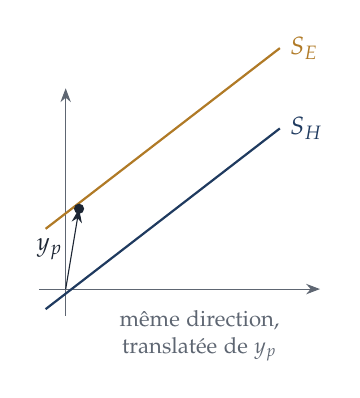
\begin{tikzpicture}[scale=0.85]
  \draw[->,Gris] (-0.4,0)--(3.8,0); \draw[->,Gris] (0,-0.4)--(0,3);
  \draw[Bleu,thick] (-0.3,-0.3)--(3.2,2.4) node[right,font=\small]{$S_H$};
  \draw[Ocre,thick] (-0.3,0.9)--(3.2,3.6) node[right,font=\small]{$S_E$};
  \draw[->,Ink] (0,0)--(0.2,1.2) node[midway,left,font=\small]{$y_p$};
  \node[pt] at (0.2,1.2){};
  \node[font=\footnotesize,Gris,align=center] at (2,-0.7) {même direction,\\ translatée de $y_p$};
\end{tikzpicture}
\end{columns}
\begin{RETENIR}
Résoudre $=$ \textbf{(1)} résoudre $(H)$ \quad\textbf{(2)} trouver \emph{une} solution particulière. Les deux problèmes sont séparés.
\end{RETENIR}
\end{frame}

\begin{frame}{Le théorème de Cauchy linéaire}
\begin{PROP}[Théorème de Cauchy linéaire \livre{th.~1.3}]
Soit $t_0\in I$. Ordre 1 : pour tout $y_0$, une \alert{unique} solution de $(E)$ sur $I$ telle que $y(t_0)=y_0$.\\
Ordre 2 : pour tous $y_0,y_1$, une \alert{unique} solution de $(E)$ sur $I$ telle que $y(t_0)=y_0$ et $y'(t_0)=y_1$.
\end{PROP}
{\footnotesize\color{Gris}Démonstration hors programme au second ordre. Hypothèse essentielle : équation \emph{normalisée} sur $I$.}\vspace{-3pt}
\pause
\begin{PROP}[Conséquences \livre{cor.~1.4}]
\begin{itemize}
\item Une solution de $(H)$ telle que $h(t_0)=h'(t_0)=0$ est la fonction nulle.
\item $\Phi:h\mapsto\big(h(t_0),h'(t_0)\big)$ est un isomorphisme de $S_H$ sur $\K^2$ : \quad $\dim S_H=2$ \ (et $1$ au premier ordre).
\end{itemize}
\end{PROP}
\pause
\begin{RETENIR}
Au second ordre, \textbf{deux solutions de $(H)$ non proportionnelles} engendrent $S_H$.
Doute ? $\dt{y_1(t_0)&y_2(t_0)\\y_1'(t_0)&y_2'(t_0)}\neq0$ \ (chapitre Déterminants).
\end{RETENIR}
\end{frame}

% ---------------------------------------------------------------- EXERCICE 1
\begin{frame}{\badgeexo{1}Retrouver toutes les solutions sans l'équation}
\begin{ENONCE}[5 min]
Les trois fonctions \ $y_1(t)=t$, \ $y_2(t)=t+e^{t}$, \ $y_3(t)=t+e^{-t}$ \ sont solutions sur $\R$ d'une même équation $(E)$ : $y''+a(t)y'+b(t)y=c(t)$, avec $a,b,c$ continues.
\begin{enumerate}
\item Sans chercher $(E)$, déterminer toutes ses solutions.
\item Déterminer la solution telle que $y(0)=1$ et $y'(0)=0$.
\item \emph{Bonus :} trouver une équation $(E)$ qui convient.
\end{enumerate}
\objectif{utiliser la structure $S_E=y_p+S_H$ et la dimension de $S_H$.}
\end{ENONCE}
\pause
\begin{INDICE}
Que dire de $y_2-y_1$ et de $y_3-y_1$ ?
\end{INDICE}
\end{frame}

\begin{frame}{\badgecor{1}Retrouver toutes les solutions sans l'équation}
\begin{columns}[T]
\column{0.42\textwidth}
\begin{RAIS}
Deux solutions de $(E)$ diffèrent d'une solution de $(H)$. On obtient ainsi deux éléments de $S_H$ ; s'ils ne sont pas
proportionnels, ils engendrent le plan $S_H$.
\end{RAIS}
\begin{OUTIL}
$S_E=y_p+S_H$ (prop.~1.2) et $\dim S_H=2$ (cor.~1.4).
\end{OUTIL}
\column{0.55\textwidth}
\etape{1.} $y_2-y_1=e^t$ et $y_3-y_1=e^{-t}$ sont dans $S_H$, et ne sont pas proportionnelles.\\
Donc $S_H=\{Ae^t+Be^{-t}\}$ et
\[S_E=\big\{t+Ae^t+Be^{-t},\ (A,B)\in\R^2\big\}.\]
\pause
\etape{2.} $y(0)=A+B=1$, $y'(0)=1+A-B=0$ : $A=0$, $B=1$.\\
La solution est $y_3$ : \ $y=t+e^{-t}$.\\[3pt]
\pause
\etape{3.} $e^t$, $e^{-t}$ solutions de $y''-y=0$ ; et $y_1''-y_1=-t$.\\
$(E)$ : $y''-y=-t$ convient.
\end{columns}
\begin{ASTU}
Toujours fixer les constantes \emph{après} avoir écrit la solution générale complète.
\end{ASTU}
\end{frame}

% =====================================================================
\partie{1.2}{Premier ordre, recollement}{Comment résoudre $y'+a(t)y=b(t)$, et que faire quand le coefficient de $y'$ s'annule ?}{\rmI}

\begin{frame}{L'équation homogène du premier ordre}
\begin{PROP}[Théorème \livre{th.~1.5}]
$A$ primitive de $a$ sur $I$. Les solutions de $y'+a(t)y=0$ sur $I$ sont les
\[t\mapsto Ke^{-A(t)},\qquad K\in\K.\]
\end{PROP}
\pause
\textbf{Preuve en une ligne :} $\big(y\,e^{A}\big)'=(y'+ay)\,e^{A}=0$ sur l'\emph{intervalle} $I$, donc $y\,e^{A}$ est constante.
\pause
\begin{columns}[T]
\column{0.5\textwidth}
\begin{EX}
$ty'+y=0$ sur $\R_+^*$ : $a(t)=\frac1t$, $A=\ln t$,\\ $y=\frac Kt$.\\
$y'-2ty=0$ : $y=Ke^{t^2}$ (signe !).
\end{EX}
\column{0.46\textwidth}
\begin{PIEGE}
Normaliser \emph{avant} de prendre la primitive.\\
$y'=a(t)y$ donne $Ke^{+A(t)}$.
\end{PIEGE}
\end{columns}
\end{frame}

\begin{frame}{Trouver une solution particulière}
\begin{METH}{Solution particulière au premier ordre \livre{méth.~1.1}}
\begin{enumerate}
\item \textbf{Évidente} : une constante, un polynôme de bas degré.
\item \textbf{$a$ constant, second membre $P(t)e^{mt}$} : $y=Q(t)e^{mt}$ ; $\deg Q=\deg P$ si $m\neq-a$, \ $\deg P+1$ si $m=-a$.\\
$\cos\omega t$, $\sin\omega t$ : résoudre avec $e^{i\omega t}$, prendre $\operatorname{Re}$ ou $\operatorname{Im}$.
\item \textbf{Variation de la constante} : $y=\lambda(t)e^{-A(t)}$. Il reste toujours
\[\lambda'(t)=b(t)\,e^{A(t)}.\]
\end{enumerate}
\end{METH}
\pause
\begin{EX}[Passage aux complexes]
$y'-3y=-7\sin4t$ : \ $z=\nu e^{4it}$, $(4i-3)\nu=-7$, $\nu=\frac{21+28i}{25}$ ;\quad
$y_p=\operatorname{Im}z=\frac{28}{25}\cos4t+\frac{21}{25}\sin4t$.
\end{EX}
\end{frame}

\begin{frame}{La variation de la constante, sur un exemple}
\begin{columns}[T]
\column{0.55\textwidth}
\textbf{Résoudre} $ty'+y=\ln t$ sur $\R_+^*$.\\[4pt]
\etape{1.} Normaliser : $y'+\frac1ty=\frac{\ln t}t$.\\[2pt]
\etape{2.} Homogène : $y=\frac Kt$.\\[2pt]
\pause
\etape{3.} On pose $y=\frac{\lambda(t)}t$ :
\[y'+\frac yt=\frac{\lambda'}t-\frac\lambda{t^2}+\frac\lambda{t^2}=\frac{\lambda'}t.\]
Donc $\lambda'=\ln t$, \ $\lambda=t\ln t-t$.\\[2pt]
\pause
\etape{4.} $S_E=\left\{\ln t-1+\dfrac Kt,\ K\in\R\right\}$.
\column{0.4\textwidth}
\begin{RETENIR}
Les termes en $\lambda$ (non dérivé) se simplifient \emph{toujours} : c'est un contrôle de calcul.
\end{RETENIR}
\begin{ASTU}
Primitive non usuelle : l'écrire $\int_{t_0}^t$, avec $t_0$ choisi pour que la condition initiale soit simple.
\end{ASTU}
\end{columns}
\end{frame}

% ---------------------------------------------------------------- EXERCICE 2
\begin{frame}{\badgeexo{2}Choisir la bonne forme}
\begin{ENONCE}[6 min]
Résoudre sur $\R$ :
\begin{enumerate}
\item $y'+y=e^{-t}$ ;
\item $y'-2ty=e^{t^2}$, avec $y(0)=1$ ;
\item $y'+y=\cos t$.
\end{enumerate}
\objectif{reconnaître, avant de calculer, laquelle des trois méthodes s'applique.}
\end{ENONCE}
\pause
\begin{INDICE}
(a) $m=-1=-a$ : que donne $Ce^{-t}$ ?\quad (b) Le second membre ressemble à la solution homogène.\quad (c) $e^{it}$.
\end{INDICE}
\end{frame}

\begin{frame}{\badgecor{2}Choisir la bonne forme}
\begin{columns}[T]
\column{0.4\textwidth}
\begin{RAIS}
Quand le second membre est \emph{solution de l'équation homogène}, la forme « comme le second membre » échoue : on monte d'un
degré, ou l'on fait varier la constante.
\end{RAIS}
\begin{OUTIL}
Méthode~1.2 : solution évidente, forme $Q(t)e^{mt}$, variation de la constante.
\end{OUTIL}
\column{0.57\textwidth}
\etape{(a)} $Ce^{-t}$ est solution de $(H)$ : on cherche $y=(\alpha t+\beta)e^{-t}$, il reste $\alpha=1$ : $y=(t+K)e^{-t}$.\\[3pt]
\pause
\etape{(b)} Homogène : $Ke^{t^2}$. Variation : $y=\lambda e^{t^2}$, $\lambda'=e^{t^2}e^{-t^2}=1$.\\
$y=(t+K)e^{t^2}$ ; $y(0)=1$ : \ $y=(t+1)e^{t^2}$.\\[3pt]
\pause
\etape{(c)} $z'+z=e^{it}$ : $z=\frac{e^{it}}{1+i}=\frac{(1-i)e^{it}}2$, \ $y_p=\operatorname{Re}z=\frac{\cos t+\sin t}2$.\\
$y=\frac{\cos t+\sin t}2+Ke^{-t}$.\\[2pt]
{\footnotesize\color{Gris}$Ke^{-t}\to0$ : toutes les solutions rejoignent la solution périodique (problème~1 de la sélection).}
\end{columns}
\end{frame}

\begin{frame}{Inconnue sous une intégrale : dériver}
\begin{METH}{Équation intégrale \livre{méth.~1.2}}
Si $f$ apparaît sous $\int_{x_0}^x$ : le membre de droite est dérivable, donc $f$ aussi ; \textbf{dériver}, et lire la condition
initiale en $x=x_0$. Conclure par équivalence (ou vérifier).
\end{METH}
\pause
\begin{EX}
$f$ continue et $f(x)=1+\displaystyle\int_0^xtf(t)\,dt$ pour tout $x$.
\begin{itemize}
\item $f$ est dérivable et $f'(x)=xf(x)$ ; en $x=0$ : $f(0)=1$.
\item Réciproquement, une solution de ce problème de Cauchy, intégrée de $0$ à $x$, vérifie l'équation.
\item Premier ordre (§1.2) : $f(x)=e^{x^2/2}$.
\end{itemize}
\end{EX}
{\small\color{Gris}Variante avec $1+x$ au lieu de $1$ : exercice~14 du TD.}
\end{frame}

\begin{frame}{Quand le coefficient de $y'$ s'annule : recoller}
\begin{METH}{Recoller des solutions en $t_0$, où $\alpha(t_0)=0$ \livre{méth.~1.3}}
\begin{enumerate}
\item Résoudre sur chaque intervalle où $\alpha\neq0$ : constantes $K_-$ et $K_+$.
\item \textbf{Continuité} en $t_0$ : limites finies et égales.
\item \textbf{Dérivabilité} en $t_0$ : limites des taux d'accroissement égales.
\item Vérifier l'équation \emph{au point} $t_0$.
\end{enumerate}
\end{METH}
\pause
\begin{columns}[T]
\column{0.32\textwidth}
\begin{EX}[$ty'+y=1$]
$1+\frac{K_\pm}t$ ; continuité : $K_\pm=0$.\\ \textbf{Une} solution : $y=1$.
\end{EX}
\column{0.32\textwidth}
\begin{EX}[$ty'-y=t^2$]
$t^2+K_\pm t$ ; taux : $K_\pm$.\\ \textbf{Une infinité} : $t^2+Kt$.
\end{EX}
\column{0.32\textwidth}
\begin{EX}[$ty'=1$]
$\ln|t|+K_\pm$, pas de limite.\\ \textbf{Aucune} solution.
\end{EX}
\end{columns}
{\small Le théorème de Cauchy ne s'applique pas en $t_0$ : tout peut arriver.}
\end{frame}

% ---------------------------------------------------------------- EXERCICE 3
\begin{frame}{\badgeexo{3}Combien de solutions sur $\R$ ?}
\begin{ENONCE}[8 min]
Déterminer les solutions sur $\R$ de chacune des équations
\[\text{(a)}\quad 2ty'-y=0\qquad\qquad\text{(b)}\quad ty'-2y=0.\]
Dans chaque cas, l'ensemble obtenu est-il une droite vectorielle, comme le « prévoit » le premier ordre ?
\objectif{appliquer les quatre étapes du recollement, et voir que Cauchy ne dit rien en $0$.}
\end{ENONCE}
\pause
\begin{INDICE}
Sur $\R_+^*$ et $\R_-^*$ : (a) $K_\pm\sqrt{|t|}$, \ (b) $K_\pm t^2$. Étudier ensuite $\dfrac{y(t)}t$ quand $t\to0$.
\end{INDICE}
\end{frame}

\begin{frame}{\badgecor{3}Combien de solutions sur $\R$ ?}
\begin{columns}[T]
\column{0.38\textwidth}
\begin{RAIS}
Deux constantes indépendantes de part et d'autre ; le raccord en $0$ impose (ou non) des conditions.
\end{RAIS}
\begin{OUTIL}
Méthode~1.3 : continuité, dérivabilité, équation en $t_0$.
\end{OUTIL}
\centering
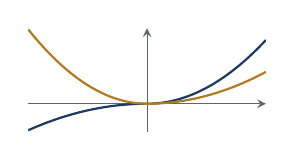
\begin{tikzpicture}
\begin{axis}[width=4.6cm,height=2.9cm,axis lines=middle,xmin=-1.5,xmax=1.5,ymin=-0.6,ymax=1.6,xtick=\empty,ytick=\empty,
  axis line style={Gris},samples=100]
\addplot[Bleu,thick,domain=0:1.5]{0.6*x^2};
\addplot[Bleu,thick,domain=-1.5:0]{-0.25*x^2};
\addplot[Ocre,thick,domain=0:1.5]{0.3*x^2};
\addplot[Ocre,thick,domain=-1.5:0]{0.7*x^2};
\end{axis}
\end{tikzpicture}\\[-2pt]{\scriptsize\color{Gris}(b) : on raccorde n'importe quelles branches}
\column{0.59\textwidth}
\etape{(a)} Sur $\R_\pm^*$ : $y=K_\pm\sqrt{|t|}$ ; continuité : $y(0)=0$. Le taux $\frac{y(t)}t=\pm\frac{K_\pm}{\sqrt{|t|}}$
n'a de limite finie que si $K_\pm=0$ : \textbf{seule la fonction nulle}.\\[3pt]
\pause
\etape{(b)} Sur $\R_\pm^*$ : $y=K_\pm t^2$. Tend vers $0$ ; taux $K_\pm t\to0$ : dérivable, $y'(0)=0$.\\
En $0$ : $0-0=0$. \ \textbf{Toutes} les fonctions égales à $K_+t^2$ sur $\R_+$ et à $K_-t^2$ sur $\R_-$ conviennent :
un \emph{plan} vectoriel.
\begin{PIEGE}
« Premier ordre $\Rightarrow$ droite » : seulement si l'équation est normalisée sur tout l'intervalle.
\end{PIEGE}
\end{columns}
\end{frame}

% =====================================================================
\partie{1.3}{Second ordre, coefficients constants}{Comment résoudre $y''+ay'+by=c(t)$ quand $a$ et $b$ sont des constantes ?}{\rmI}

\begin{frame}{L'équation caractéristique}
\textbf{Idée :} chercher des solutions $e^{rt}$ de $y''+ay'+by=0$ :
\[(e^{rt})''+a(e^{rt})'+b\,e^{rt}=(r^2+ar+b)\,e^{rt}=0\iff r^2+ar+b=0.\]
\pause
\begin{PROP}[Théorème \livre{th.~1.11}]
\begin{tabular}{@{}lll@{}}
\textbf{Cas complexe} & $r_1\neq r_2$ : $Ae^{r_1t}+Be^{r_2t}$ & racine double $r$ : $(A+Bt)e^{rt}$\\[3pt]
\textbf{Cas réel}, $\Delta=a^2-4b$ & $\Delta>0$ : $Ae^{r_1t}+Be^{r_2t}$ & $\Delta=0$ : $(A+Bt)e^{rt}$\\
& \multicolumn{2}{l}{$\Delta<0$, $r=\alpha\pm i\beta$ : \ $e^{\alpha t}\big(A\cos\beta t+B\sin\beta t\big)$, \quad $A,B\in\R$}
\end{tabular}
\end{PROP}
\pause
{\small\textbf{Pourquoi $te^{rt}$ ?} Avec $y=z\,e^{rt}$ : $y''+ay'+by=\big(z''+(2r+a)z'\big)e^{rt}$. Racine double : $2r+a=0$, donc $z''=0$,
$z=A+Bt$. Les deux solutions sont non proportionnelles : elles engendrent le plan $S_H$.}
\end{frame}

% ---------------------------------------------------------------- EXERCICE 4
\begin{frame}{\badgeexo{4}Un oscillateur amorti}
\begin{ENONCE}[4 min]
Déterminer la solution réelle de
\[y''+4y'+13y=0,\qquad y(0)=0,\quad y'(0)=3,\]
puis décrire son allure quand $t\to+\infty$.
\objectif{appliquer le théorème dans le cas $\Delta<0$, puis la condition de Cauchy.}
\end{ENONCE}
\end{frame}

\begin{frame}{\badgecor{4}Un oscillateur amorti}
\begin{columns}[T]
\column{0.5\textwidth}
\etape{1.} $r^2+4r+13=0$, \ $\Delta=-36$, \ $r=-2\pm3i$.\\
$y=e^{-2t}(A\cos3t+B\sin3t)$.\\[3pt]
\pause
\etape{2.} $y(0)=A=0$ ; \ $y'(0)=-2A+3B=3$, \ $B=1$.
\[y=e^{-2t}\sin3t.\]
\pause
\etape{3.} Pulsation $3$, amplitude $e^{-2t}\to0$ : régime \emph{pseudo-périodique}.
\begin{RAIS}[À retenir de la correction]
Partie réelle des racines $\to$ amortissement ;\\ partie imaginaire $\to$ pulsation.
\end{RAIS}
\column{0.45\textwidth}
\centering
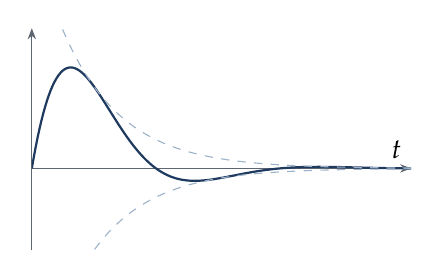
\begin{tikzpicture}
\begin{axis}[width=6.4cm,height=4.4cm,axis lines=middle,xmin=0,xmax=3.2,ymin=-0.35,ymax=0.6,xtick=\empty,ytick=\empty,
  axis line style={Gris,-{Stealth[length=4pt]}},samples=200,xlabel={$t$}]
\addplot[Bleu,thick,domain=0:3.2]{exp(-2*x)*sin(3*x)};
\addplot[BleuClair,dashed,domain=0:3.2]{exp(-2*x)};
\addplot[BleuClair,dashed,domain=0:3.2]{-exp(-2*x)};
\end{axis}
\end{tikzpicture}
\end{columns}
\end{frame}

\begin{frame}{Second membre $P(t)e^{mt}$}
\begin{METH}{Solution particulière \livre{méth.~1.4}}
Chercher $y=Q(t)e^{mt}$, avec \ $\deg Q=\deg P+\big(\text{multiplicité de $m$ comme racine : }0,\ 1\text{ ou }2\big)$.\\[2pt]
En reportant :\qquad $Q''+(2m+a)Q'+(m^2+am+b)Q=P.$
\end{METH}
\pause
\begin{columns}[T]
\column{0.5\textwidth}
\begin{ASTU}
$m$ non racine : les trois termes.\\ $m$ racine simple : plus de terme en $Q$.\\ $m$ racine double : $Q''=P$.
\end{ASTU}
\column{0.46\textwidth}
\begin{RETENIR}
$\cos\omega t$, $e^{\alpha t}\sin\omega t$ : passer par $e^{(\alpha+i\omega)t}$, puis $\operatorname{Re}$ ou $\operatorname{Im}$.\\
Second membre somme : superposition.
\end{RETENIR}
\end{columns}
\pause
\begin{EX}[Superposition]
$y''-3y'+2y=2t+3+e^t$ (racines $1$ et $2$). \ $2t+3$ : $y_1=t+3$. \ $e^t$ ($m=1$ simple) : $Q''-Q'=1$, $y_2=-te^t$.\\
$y=t+3-te^t+Ae^t+Be^{2t}$.
\end{EX}
\end{frame}

\begin{frame}{Résonance et oscillateur amorti}
\begin{columns}[T]
\column{0.5\textwidth}
\begin{EX}[Résonance]
$y''+y=\sin t$ : $i$ racine simple, $z=Q(t)e^{it}$ avec $Q''+2iQ'=1$, $Q=-\frac i2t$.\\
$y_p=\operatorname{Im}z=-\frac t2\cos t$ : l'amplitude \alert{croît sans limite}.
\end{EX}
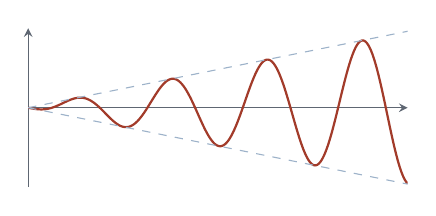
\begin{tikzpicture}
\begin{axis}[width=6.4cm,height=3.6cm,axis lines=middle,xmin=0,xmax=25,ymin=-13,ymax=13,xtick=\empty,ytick=\empty,
  axis line style={Gris},samples=300]
\addplot[Brique,thick,domain=0:25]{-x/2*cos(x)};
\addplot[BleuClair,dashed,domain=0:25]{x/2};\addplot[BleuClair,dashed,domain=0:25]{-x/2};
\end{axis}
\end{tikzpicture}
\column{0.46\textwidth}
\begin{PROP}[Oscillateur $y''+2\lambda y'+\omega^2y=0$]
$\lambda,\omega>0$, discriminant réduit $\lambda^2-\omega^2$ :
\begin{itemize}
\item $\lambda>\omega$ : apériodique ;
\item $\lambda=\omega$ : critique ;
\item $\lambda<\omega$ : pseudo-périodique, pulsation $\sqrt{\omega^2-\lambda^2}$, amortie par $e^{-\lambda t}$.
\end{itemize}
\end{PROP}
{\footnotesize\color{Gris}Le vocabulaire des sciences physiques, avec les outils du cours.}
\end{columns}
\end{frame}

% ---------------------------------------------------------------- EXERCICE 5
\begin{frame}{\badgeexo{5}Quelle forme pour la solution particulière ?}
\begin{ENONCE}[8 min]
Pour chaque équation, donner la \emph{forme} de la solution particulière à chercher, puis la calculer.
\[\text{(a)}\ \ y''-y=te^t\qquad\text{(b)}\ \ y''+2y'+y=e^{-t}\qquad\text{(c)}\ \ y''+y=\cos2t\]
\objectif{lire la multiplicité de $m$, puis utiliser $Q''+(2m+a)Q'+(m^2+am+b)Q=P$.}
\end{ENONCE}
\pause
\begin{INDICE}
Racines : (a) $\pm1$ ; (b) $-1$ double ; (c) $\pm i$. Comparer avec $m=1$, $m=-1$, $m=2i$.
\end{INDICE}
\end{frame}

\begin{frame}{\badgecor{5}Quelle forme pour la solution particulière ?}
\begin{columns}[T]
\column{0.38\textwidth}
\begin{RAIS}
On ne calcule rien avant d'avoir comparé $m$ aux racines : c'est la multiplicité qui fixe $\deg Q$.
\end{RAIS}
\begin{OUTIL}
Méthode~1.4 : $\deg Q=\deg P+$ multiplicité.
\end{OUTIL}
\column{0.59\textwidth}
\etape{(a)} $m=1$ racine simple, $\deg Q=2$. $a=0$, $b=-1$ : $Q''+2Q'=t$.\\
$Q=\frac{t^2}4-\frac t4$, \ $y_p=\left(\frac{t^2}4-\frac t4\right)e^t$.\\[3pt]
\pause
\etape{(b)} $m=-1$ racine double : $Q''=1$, $Q=\frac{t^2}2$, \ $y_p=\frac{t^2}2e^{-t}$.\\[3pt]
\pause
\etape{(c)} $m=2i$ non racine : $z=Ce^{2it}$, $(-4+1)C=1$, \ $y_p=\operatorname{Re}z=-\frac13\cos2t$.
\end{columns}
\begin{PIEGE}
En (b), chercher $Ce^{-t}$ ou $Cte^{-t}$ conduit à $0=1$ : ce sont des solutions de $(H)$.
\end{PIEGE}
\end{frame}

\begin{frame}{Second membre quelconque : variation de la constante}
\begin{METH}{Variation de la constante au second ordre \livre{méth.~1.5}}
Prendre $\varphi$ solution de $(H)$ \alert{qui ne s'annule pas} sur $I$ (souvent $e^{rt}$) et chercher $y=\lambda(t)\varphi(t)$.
Le terme en $\lambda$ disparaît : il reste une équation du \emph{premier ordre} en $\lambda'$.
\end{METH}
\pause
\begin{EX}
$y''-2y'+y=\dfrac{2te^t}{1+t^2}$. Racine double $1$, $\varphi=e^t$. Avec $y=\lambda e^t$ : \ $y''-2y'+y=\lambda''e^t$.
\[\lambda''=\frac{2t}{1+t^2},\quad\lambda'=\ln(1+t^2)+C,\quad\lambda=t\ln(1+t^2)-2t+2\arctan t+Ct+D.\]
\end{EX}
{\small\color{Gris}Autre exemple : $y''+y=\frac1{\cos t}$ avec $\varphi=\cos$ sur $\left]-\frac\pi2,\frac\pi2\right[$ (exercice~13 du TD).}
\end{frame}

% =====================================================================
\partie{1.4}{Second ordre, coefficients continus}{Plus de formule : comment trouver deux solutions non proportionnelles ?}{\rmI}

\begin{frame}{Le principe}
$(E)$ : $\alpha(t)y''+\beta(t)y'+\gamma(t)y=\delta(t)$, avec $\alpha$ \alert{qui ne s'annule pas} sur $I$.
\begin{itemize}
\item Cauchy et la structure restent vrais : $\dim S_H=2$.
\item Il n'y a \alert{plus de formule générale}. Il faut \textbf{deux solutions non proportionnelles} de $(H)$, puis une solution particulière.
\item Le programme prévoit des résolutions \emph{guidées} : \textbf{l'énoncé indique la méthode}.
\end{itemize}
\pause
\begin{center}
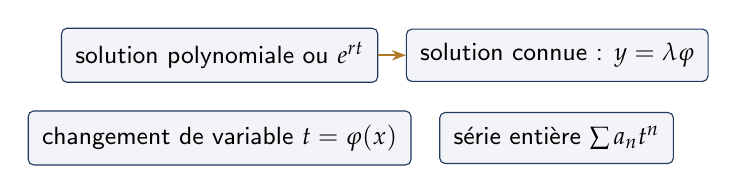
\begin{tikzpicture}[node distance=0.35cm,every node/.style={font=\sffamily\small}]
\node[draw=Bleu,fill=Fond,rounded corners=2pt,inner sep=5pt](a){solution polynomiale ou $e^{rt}$};
\node[draw=Bleu,fill=Fond,rounded corners=2pt,inner sep=5pt,right=of a](b){solution connue : $y=\lambda\varphi$};
\node[draw=Bleu,fill=Fond,rounded corners=2pt,inner sep=5pt,below=of a](c){changement de variable $t=\varphi(x)$};
\node[draw=Bleu,fill=Fond,rounded corners=2pt,inner sep=5pt,right=of c](d){série entière $\sum a_nt^n$};
\draw[->,Ocre,thick] (a)--(b);
\end{tikzpicture}\\[2pt]
{\footnotesize\color{Gris}une première solution trouvée permet souvent d'obtenir la seconde}
\end{center}
\end{frame}

\begin{frame}{Solution polynomiale, solution exponentielle}
\begin{METH}{Chercher une solution polynomiale ou exponentielle \livre{méth.~1.6}}
\textbf{Polynôme} $y=\sum_{k=0}^na_kt^k$, $a_n\neq0$ : le coefficient de $t^n$ doit être nul, cela fixe $n$ ; puis identifier.\\
\textbf{Exponentielle} $y=e^{rt}$ : l'égalité a lieu pour \emph{tout} $t$ : coefficient de $t$ et constante nuls.
\end{METH}
\pause
\begin{EX}
$(2t+1)y''+(4t-2)y'-8y=0$.
\begin{itemize}
\item Degré $n$ : coefficient de $t^n$ : $(4n-8)a_n=0$, donc $n=2$ ; on trouve $y_1=4t^2+1$.
\item $e^{rt}$ : $(2r^2+4r)t+(r^2-2r-8)=0$ pour tout $t$ : $r=-2$, \ $y_2=e^{-2t}$.
\item Non proportionnelles : $S_H=\{A(4t^2+1)+Be^{-2t}\}$ sur tout intervalle ne contenant pas $-\frac12$.
\end{itemize}
\end{EX}
\end{frame}

% ---------------------------------------------------------------- EXERCICE 6
\begin{frame}{\badgeexo{6}Deux polynômes solutions}
\begin{ENONCE}[6 min]
On considère $(H)$ : $(t^2+1)y''-2ty'+2y=0$ sur $\R$.
\begin{enumerate}
\item Quels degrés peut avoir une solution polynomiale non nulle ?
\item En déduire toutes les solutions de $(H)$ sur $\R$.
\end{enumerate}
\objectif{la condition sur le coefficient dominant, puis la structure (dimension 2).}
\end{ENONCE}
\pause
\begin{INDICE}
Coefficient de $t^n$ : $n(n-1)-2n+2$. Factoriser.
\end{INDICE}
\end{frame}

\begin{frame}{\badgecor{6}Deux polynômes solutions}
\begin{columns}[T]
\column{0.4\textwidth}
\begin{RAIS}
Le terme dominant donne les degrés possibles ; deux polynômes de degrés différents ne sont pas proportionnels : on a tout
$S_H$.
\end{RAIS}
\begin{OUTIL}
Méthode~1.6, puis cor.~1.4 : $\dim S_H=2$ ($t^2+1\neq0$ sur $\R$).
\end{OUTIL}
\column{0.57\textwidth}
\etape{1.} Coefficient de $t^n$ : $\big(n(n-1)-2n+2\big)a_n=(n-1)(n-2)a_n$.\\
Donc $n=1$ ou $n=2$.\\[3pt]
\pause
\etape{2.} $y=at^2+bt+c$ : $(t^2+1)2a-2t(2at+b)+2(at^2+bt+c)=2a+2c=0$.\\
Donc $c=-a$ : \ $y=a(t^2-1)+bt$.\\[3pt]
\pause
$t$ et $t^2-1$ ne sont pas proportionnelles, et $\dim S_H=2$ :
\[S_H=\big\{a(t^2-1)+bt,\ (a,b)\in\R^2\big\}.\]
\end{columns}
\begin{ASTU}
On n'a pas besoin de résoudre autre chose : la dimension garantit qu'il n'y a pas d'autre solution.
\end{ASTU}
\end{frame}

\begin{frame}{Une solution connue : abaisser l'ordre}
\begin{METH}{Une solution $\varphi$ de $(H)$ ne s'annulant pas est connue \livre{méth.~1.7}}
Chercher $y=\lambda(t)\varphi(t)$. Le terme en $\lambda$ disparaît (car $\varphi$ est solution) :
\[\alpha\varphi\,\lambda''+(2\alpha\varphi'+\beta\varphi)\,\lambda'=\delta\quad:\quad\text{premier ordre en }\mu=\lambda'.\]
\end{METH}
\pause
\begin{EX}[$t^2y''-2y=3t^2$ sur $\R_+^*$]
\etape{1.} Polynôme solution de $(H)$ : $n(n-1)-2=0$, $n=2$ : $\varphi=t^2$.\\
\etape{2.} $y=\lambda t^2$ : $t^4\lambda''+4t^3\lambda'=3t^2$, soit $\mu'+\frac4t\mu=\frac3{t^2}$.\\
\etape{3.} $\mu=\frac1t+\frac K{t^4}$, \ $\lambda=\ln t-\frac K{3t^3}+D$.\qquad $y=t^2\ln t+\dfrac at+bt^2$.
\end{EX}
\end{frame}

\begin{frame}{Changement de variable}
\begin{METH}{Changement de variable \livre{méth.~1.8}}
$t=\varphi(x)$, bijection $\mathcal C^2$ de réciproque $\mathcal C^2$ ; \ $z(x)=y(\varphi(x))$,
\[z'(x)=\varphi'(x)\,y'(\varphi(x)),\qquad z''(x)=\varphi'(x)^2\,y''(\varphi(x))+\varphi''(x)\,y'(\varphi(x)).\]
L'équation en $z$ doit devenir connue ; on revient à $y=z\circ\varphi^{-1}$.
\end{METH}
\pause
\begin{columns}[T]
\column{0.5\textwidth}
\begin{EX}[$t=\cos x$]
$(1-t^2)y''-ty'+y=0$ sur $]-1,1[$ devient $z''+z=0$ :\\ $y=At+B\sqrt{1-t^2}$.
\end{EX}
\column{0.46\textwidth}
\begin{EX}[Euler, $t=e^x$]
$t^2y''=z''-z'$, \ $ty'=z'$ :\\ coefficients constants (exercice~20 du TD).
\end{EX}
\end{columns}
{\small\color{Gris}Variante : \emph{changement de fonction} $z=ty$, $z=t^2y$\dots\ proposé par l'énoncé (exercices~25 et 27 du TD).}
\end{frame}

\begin{frame}{Solutions développables en série entière}
\begin{METH}{Analyse, puis synthèse \livre{méth.~1.9}}
\textbf{Analyse :} $y=\sum a_nt^n$ de rayon $R>0$ ; dériver terme à terme, \emph{décaler les indices} pour tout écrire en $t^n$,
identifier : relation de récurrence.\\
\textbf{Synthèse :} calculer les $a_n$, le rayon ; la somme est solution sur $]-R,R[$. Reconnaître une fonction usuelle.
\end{METH}
\pause
\begin{EX}[$(t^2+t)y''+(3t+1)y'+y=0$]
Coefficient de $t^n$ : $(n+1)^2(a_{n+1}+a_n)=0$, donc $a_n=(-1)^na_0$, rayon $1$ : \ $y=\dfrac{a_0}{1+t}$ sur $]-1,1[$.
\end{EX}
\pause
\begin{PIEGE}
Une série entière ne donne en général \emph{qu'une partie} de $S_H$, et seulement sur $]-R,R[$.
\end{PIEGE}
\end{frame}

% ---------------------------------------------------------------- EXERCICE 7
\begin{frame}{\badgeexo{7}Une série entière qui donne tout}
\begin{ENONCE}[8 min]
On considère $(H)$ : $(1-t^2)y''-4ty'-2y=0$ sur $]-1,1[$.
\begin{enumerate}
\item Déterminer les solutions développables en série entière, et leur rayon de convergence.
\item Exprimer leur somme à l'aide de fonctions usuelles.
\item En déduire toutes les solutions de $(H)$ sur $]-1,1[$.
\end{enumerate}
\objectif{décaler les indices, identifier, puis conclure avec la dimension.}
\end{ENONCE}
\pause
\begin{INDICE}
$t^2y''=\sum n(n-1)a_nt^n$ et $y''=\sum(n+2)(n+1)a_{n+2}t^n$. La relation lie $a_{n+2}$ et $a_n$.
\end{INDICE}
\end{frame}

\begin{frame}{\badgecor{7}Une série entière qui donne tout}
\begin{columns}[T]
\column{0.38\textwidth}
\begin{RAIS}
Analyse : récurrence d'ordre 2 sur les indices, donc \emph{deux} constantes libres $a_0$, $a_1$. Synthèse : rayon, puis somme.
\end{RAIS}
\begin{OUTIL}
Méthode~1.9 ; cor.~1.4 ($1-t^2\neq0$ sur $]-1,1[$).
\end{OUTIL}
\column{0.59\textwidth}
\etape{1.} Coefficient de $t^n$ : $(n+2)(n+1)a_{n+2}-(n^2+3n+2)a_n$,\\ soit $(n+1)(n+2)(a_{n+2}-a_n)$.\\[2pt]
Donc $a_{n+2}=a_n$ : \ $a_{2p}=a_0$, $a_{2p+1}=a_1$. Rayon $1$ (si $(a_0,a_1)\neq(0,0)$).\\[3pt]
\pause
\etape{2.} $y=a_0\sum t^{2p}+a_1\sum t^{2p+1}=\dfrac{a_0+a_1t}{1-t^2}$.\\[3pt]
\pause
\etape{3.} $\frac1{1-t^2}$ et $\frac t{1-t^2}$ sont deux solutions non proportionnelles : \
$S_H=\left\{\dfrac{a+bt}{1-t^2}\right\}$.
\end{columns}
\begin{ASTU}
Exceptionnellement, la série entière donne tout $S_H$ : deux constantes libres.
\end{ASTU}
\end{frame}

% =====================================================================
\partie{1.5}{Quelle méthode ? Synthèse}{Devant une équation, par quoi commencer ?}{\rmI}

\begin{frame}{Quelle méthode ?}
\small
\renewcommand{\arraystretch}{1.3}
\begin{tabular}{@{}p{5.2cm}p{8.6cm}@{}}
\toprule
\textbf{Équation} & \textbf{Méthode}\\\midrule
$y'+a(t)y=b(t)$ & $Ke^{-A}$ ; solution évidente, forme du second membre, ou variation de la constante\\
$\alpha(t)y'+\dots$ avec $\alpha(t_0)=0$ & résoudre sur chaque intervalle, puis recoller\\
$y''+ay'+by=c(t)$, $a,b$ constants & équation caractéristique ; $P(t)e^{mt}$ ; sinon variation de la constante\\
$\alpha y''+\beta y'+\gamma y=\delta$ & \textbf{suivre l'indication} : polynôme, $e^{rt}$, $y=\lambda\varphi$, $t=\varphi(x)$, $z=t^ky$, série entière\\
$f$ sous $\int_{x_0}^x$ & dériver, condition initiale en $x_0$\\
$f'(x)=f(-x)$, \dots & dériver, puis vérifier la \emph{réciproque}\\\bottomrule
\end{tabular}
\end{frame}

\begin{frame}{Pièges et essentiel}
\begin{columns}[T]
\column{0.48\textwidth}
\begin{PIEGE}[Pièges fréquents]
\begin{itemize}
\item Ne pas normaliser ; signe de $e^{-A}$.
\item Oublier la résonance.
\item $\sin$ au second membre : partie \emph{imaginaire}.
\item Conditions initiales avant d'ajouter $y_p$.
\item Diviser par un coefficient qui s'annule.
\item Affirmer l'unicité d'une solution recollée.
\end{itemize}
\end{PIEGE}
\column{0.48\textwidth}
\begin{RETENIR}
\begin{itemize}
\item $S_E=y_p+S_H$ ; $\dim S_H=1$ ou $2$ si l'équation est normalisée.
\item Cauchy : une ou deux conditions en $t_0$.
\item Ordre 1 : $Ke^{-A}$ ; $\lambda'=b\,e^{A}$.
\item Constants : $r^2+ar+b=0$ ; $\deg Q=\deg P+$ multiplicité.
\item Continus : deux solutions non proportionnelles ; $y=\lambda\varphi$.
\end{itemize}
\end{RETENIR}
\end{columns}
\end{frame}

\begin{frame}{Après la séance}
\begin{columns}[T]
\column{0.5\textwidth}
\begin{enumerate}
\item \textbf{Relire le livre} (chapitre~4) : démonstrations et exemples rédigés.
\item \textbf{Apprendre la fiche} : formules, méthodes, pièges.
\item \textbf{Cinq problèmes} de la sélection, dans l'ordre :
\begin{itemize}\small
\item régimes transitoire et permanent ;
\item solution polynomiale et $t=\sh x$ ;
\item changement de fonction et recollement ;
\item trois méthodes pour une même équation ;
\item solutions périodiques d'un oscillateur forcé.
\end{itemize}
\item Puis le \textbf{TD complet} (28 exercices, quatre niveaux).
\end{enumerate}
\column{0.44\textwidth}
\begin{ASTU}[Pour chercher seul]
Lire l'en-tête du problème, chercher au brouillon, ne lire qu'\emph{une} indication en cas de blocage, la correction à la fin.
\end{ASTU}
\begin{HPBOX}
Systèmes $X'=AX$, ordre $\geq3$ : hors programme PT. L'équation d'Euler n'est traitée qu'avec l'indication $t=e^x$.
\end{HPBOX}
\end{columns}
\end{frame}

\end{document}
